\begin{name}
    {ÔN TẬP HÌNH HỌC - GIỮA KÌ II}
	{TOÁN 10}
	{LỚP TOÁN THẦY PHÁT}
	{Thời gian: 90 phút - Không kể thời gian phát đề}
\end{name}
\Opensolutionfile{ans}[ans/OTHHDTDT-10-GK2-2024-06-10]
\begin{ex}%[0H9N3-6]
Trong mặt phẳng $Oxy$, cho đường thẳng $d\colon x+y-4=0$. Điểm nào sau đây nằm trên đường thẳng $d$?
\choice
{$M(1;-3)$}
{\True $N(1;3)$}
{$P(2;1)$}
{$Q(-2;3)$}
\loigiai{
Ta có $1+3-4=0$ nên điểm là $N(1;3)$ nằm trên đường thẳng $d$.
}
\end{ex}

\begin{ex}%[0H9N3-2]%[Dự án đề kiểm tra Toán 11 GHKII NH23-24-Nguyen Tran Anh Tuan]%[THPT Thiệu Hóa - Thanh Hóa]
Trong mặt phẳng với hệ trục tọa độ $Oxy$, cho đường thẳng $d$ cắt trục $Ox$, $Oy$ lần lượt tại hai điểm $A(3; 0)$ và $B(0;-2)$. Đường thẳng $d$ có phương trình là
\choice
{$\dfrac{x}{3}-\dfrac{y}{2}=-1$}
{$\dfrac{x}{-2}+\dfrac{y}{3}=1$}
{\True $\dfrac{x}{3}-\dfrac{y}{2}=1$}
{$\dfrac{x}{3}-\dfrac{y}{2}=0$}
\loigiai{
Vì $d$ cắt hai trục $Ox$, $Oy$ lần lượt tại hai điểm $A(3; 0)$ và $B(0;-2)$ nên phương trình đoạn chắn là $d\colon \dfrac{x}{3}+\dfrac{y}{-2}=1$.\\
Vậy $d\colon \dfrac{x}{3}-\dfrac{y}{2}=1$.
}
\end{ex}

\begin{ex}%[0H9N3-1]%[Dự án đề kiểm tra Toán Khối 10 CK2 NH23-24-Dot 16- Khắc Thiên]%[THPT Chuyên Hùng Vương - Phú Thọ]
Trong mặt phẳng $Oxy$, vectơ nào dưới đây là một vectơ chỉ phương của đường thẳng song song với trục $Oy$ ?
\choice
{$\overrightarrow{u_1}=(1 ; 0)$}
{$\overrightarrow{u_4}=(1 ; 1)$}
{$\overrightarrow{u_3}=(-1 ; 1)$}
{\True $\overrightarrow{u_2}=(0 ; 1)$}
\loigiai{
Trục $Oy$ có phương trình là $x=0$.\\
Vec-tơ pháp tuyến của trục $Oy$ là $\overrightarrow{u}=(1; 0)$.\\
Do đó một vectơ chỉ phương của đường thẳng song song với trục $Oy$ là $\overrightarrow{u}=(0 ; 1)$.
}
\end{ex}

\begin{ex}%[10-11EX-GK2-2425]%[Hoàng Ngọc Lâm]%[0H9N3-1]
Trong mặt phẳng tọa độ $Oxy$, cho đường thẳng $d\colon \heva{&x=-4+5t\\&y=3-t}(t \in \mathbb{R})$. Véc-tơ nào sau đây là một véc-tơ chỉ phương của đường thẳng $d$?
\choice
{$\overrightarrow{u}_3 = (5;1)$}
{$\overrightarrow{u}_4 = (1;5)$}
{$\overrightarrow{u}_2 = (-4;3)$}
{\True $\overrightarrow{u}_1 = \left(\dfrac{5}{2}; -\dfrac{1}{2} \right)$}
\loigiai{
$d\colon \heva{&x=-4+5t\\&y=3-t}(t \in \mathbb{R})$ nên $d$ có một véc-tơ chỉ phương là $\overrightarrow{u}=(5;-1)$. Ta thấy $\overrightarrow{u}_1 = \left(\dfrac{5}{2}; -\dfrac{1}{2} \right)$ cùng phương với $\overrightarrow{u}$ nên $\overrightarrow{u}_1$ là một véc-tơ chỉ phương của $d$.
}
\end{ex}

\begin{ex}%[Dự án Đề GK2 PNL Cấu Trúc 2025]%[Đào-V- Thuỷ]%[0H9N3-1]
Toạ độ véc-tơ pháp tuyến của đường thẳng $d\colon \heva{&x=-4+3t\\ &y=1+2t}$ là
\choice
{$(1;1)$}
{$(-4;-6)$}
{\True $(2;-3)$}
{$(-3;2)$}
\loigiai
{
Đường thẳng $d\colon \heva{&x=-4+3t\\ &y=1+2t}$ có một véc-tơ chỉ phương $\vec{u}=(3;2)$. Do đó $(2;-3)$ là toạ độ một véc-tơ pháp tuyến của $d$.
}
\end{ex}

\begin{ex}%[0H9N3-2]
Trong mặt phẳng tọa độ $Oxy$, đường thẳng $d\colon \heva{&x=1-2t\\&y=-2+3t},(t \in \mathbb{R})$ có một vectơ chỉ phương là
\choice
{$1$}
{\True $1$}
{$1$}
{$1$}
\loigiai{
Đường thẳng $d$ có vectơ chỉ phương là $(-2;3)$ nên $\overrightarrow u=(4;-6)$ cũng là một vectơ chỉ phương của đường thẳng $d$.}
\end{ex}

\begin{ex}%[0H9N4-1]%[Dự án đề kiểm tra Toán 10, 11 HKII NH23-24-BCTuan]%[THPT LTV-Hà Nội]
Trong mặt phẳng tọa độ $Oxy$, cho đường tròn $(C)\colon (x-1)^2+(y-2)^2=9$. Tâm $I$ và bán kính $R$ của đường tròn là
\choice
{$I(1;2)$; $R=9$}
{$I(-1;2)$; $R=9$}
{$I(-1;-2)$; $R=3$}
{\True $I(1;2)$; $R=3$}
\loigiai{
Đường tròn $(C)$ có tâm $I(1;2)$, bán kính $R=3$.
}
\end{ex}

\begin{ex}%[0H9N4-2]%[Dự án đề kiểm tra Toán 10 HKII NH23-24- Đoàn Minh Tâm]%[THPT Mạc Đĩnh Chi]
Trong mặt phẳng tọa độ $Oxy$, đường tròn tâm $I\left(-3;1\right)$, bán kính $R=9$ có phương trình là
\choice
{$\left(x+3\right)^2+\left(y-1\right)^2=9$}
{$\left(x-3\right)^2+\left(y+1\right)^2=81$}
{\True $\left(x+3\right)^2+\left(y-1\right)^2=81$}
{$\left(x+3\right)^2+\left(y-1\right)^2=9$}
\loigiai{
Ta có đường tròn tâm $I\left(-3;1\right)$, bán kính $R=9$ có phương trình là
\[\left(x+3\right)^2+\left(y-1\right)^2=81.\]
}
\end{ex}

\begin{ex}%[0H9N4-1]%[Dự án đề kiểm tra Toán 10 CHKI NH23-24- lamnguyen]%[THPT - Đồng nai]
Tọa độ tâm I và bán kính R của đường tròn $(C)\colon {\left(x-1\right)^2}+\left(y+3\right)^2=16$ là
\choice
{$I\left(-1;3\right)$, $R=4$}
{\True $I\left(1;-3\right)$, $R=4$}
{$I\left(1;-3\right)$, $R=16$}
{$I\left(-1;3\right)$, $R=16$}
\loigiai{
Ta có đường tròn $(C):{\left(x-1\right)^2}+\left(y+3\right)^2=16$ có tâm $I\left(1;-3\right)$, $R=\sqrt{16}=4$.
}
\end{ex}

\begin{ex}%[0H9N4-1]%[Dự án đề kiểm tra Toán khối 10 HKII NH23-24-Đợt 15-Lê Hải Phụng]%[THPT Chuyên Lê Quý Đôn - HCM]
Trong mặt phẳng $Oxy$, cho đường tròn $(C)\colon{\left(x-2\right)^2}+\left(y+4\right)^2=16$. Đường tròn $(C)$có tọa độ tâm $ I$ và bán kính $ R$ bằng
\choice
{$ I\left(-2;4\right)$, $R=4$}
{\True $ I\left(2;-4\right)$, $R=4$}
{$ I\left(-2;4\right)$, $R=16$}
{$ I\left(2;-4\right)$, $R=16$}
\loigiai{}
\end{ex}

\begin{ex}%[soạn để GHK, HK]%[Huỳnh Xuân Tín]%[0H9N4-2]
Trong mặt phẳng $Oxy$, đường tròn tâm $I(3;-1)$ và bán kính $R=2$ có phương trình là
\choice
{$(x+3)^2+(y-1)^2=4$}
{$(x-3)^2+(y-1)^2=4$}
{\True $(x-3)^2+(y+1)^2=4$}
{$(x+3)^2+(y+1)^2=4$}
\loigiai{
Phương trình đường tròn có tâm $I(3;-1)$, bán kính $R=2$ là $(x-3)^2+(y+1)^2=4$.
}
\end{ex}

\begin{ex}%[0H9N4-1]%[Dự án đề kiểm tra Toán khối 10 HKII NH23-24-Đợt 15-Lê Hải Phụng]%[THPT Chuyên Lê Quý Đôn - HCM]
Trong mặt phẳng $Oxy$, phương trình đường tròn là
\choice
{\True $x^2+y^2-4x+6y-12=0$}
{$x^2+y^2-4x+2y+10=0$}
{$x^2+y^2+6=0$}
{$x^2+2y^2-4x+2y-1=0$}
\loigiai{
\begin{itemize}
\item $x^2+y^2-4x+6y-12=0$ có $a^2+b^2-c=2^2+(-3)^2-(-12) = 25>0$ nên là phương trình đường tròn.
\item $x^2+y^2-4x+2y+10=0$ có $a^2+b^2-c=2^2+(-1)^2-10 = -5<0$ nên không là phương trình đường tròn.
\item $x^2+y^2+6=0$ có $a^2+b^2-c=0^2+0^2-6 = -6<0$ nên không là phương trình đường tròn.
\item $x^2+2y^2-4x+2y-1=0$ không là phương trình đường tròn.
\end{itemize}
}
\end{ex}

\begin{ex}%[Dự án 18 - TeamTeXHoa - Huỳnh Thanh Chí]%[0H9V3-6]
Cho tam giác $ABC$ có $A(3; 2), B(1;-1), C(7;-4)$.
\choiceTF
{Độ dài đường cao kẻ từ $A$ xuống cạnh $BC$ là $\dfrac{6}{\sqrt{5}}$}
{Điểm $E\left(\dfrac{2}{37}; -\dfrac{5}{4}\right)$ là tâm đường tròn ngoại tiếp của tam giác $ABC$}
{\True Điểm $I\left(\dfrac{5}{3}; 0\right)$ là chân đường phân giác trong kẻ từ $C$ đến cạnh $AB$ của tam giác $ABC$}
{Phương trình đường thẳng đi qua $A(3; 2)$ và cắt tia $Ox$ tại $M$, cắt tia $Oy$ tại $N$ sao cho hoành độ của $M$, tung độ của $N$ đều dương và diện tích tam giác $OMN$ đạt giá trị nhỏ nhất là $2x+3y+1=0$}
\loigiai{
\begin{itemchoice}
\itemch Ta có $\overrightarrow{BC}=(7-1; 0-4+1)=(6;-3) \Rightarrow \overrightarrow{u}_{BC}=(2;-1) \Rightarrow \overrightarrow{n}_{BC}=(1; 2)$.\\
Do đó đường thẳng $BC$ có phương trình là $1\cdot (x-1)+2\cdot(y+1)=0\Leftrightarrow x+2y+1=0$.\\
Ta có độ dài đường cao kẻ từ $A$ xuống cạnh $BC$ là khoảng cách từ $A$ đến đường thẳng $BC$.\\
Khi đó $\mathrm{d}(A; BC)=\dfrac{|1\cdot 3+2\cdot 2+1|}{\sqrt{1^2+2^2}}=\dfrac{8}{\sqrt{5}}$.
\itemch Gọi $E(x;y)$ là tâm đường tròn ngoại tiếp tam giác $ABC$. Khi đó\\
$EA=EB=EC\Leftrightarrow\heva{&EA^2=EB^2\\
&EA^2=EC^2.} \quad (1)$\\
Ta có $\overrightarrow{AE}=(x-3; y-2)$; $\overrightarrow{BE}=(x-1; y+1)$; $\overrightarrow{CE}=(x-7; y+4)$.\\
Khi đó\\
$(1) \Leftrightarrow\heva{&(x-3)^2+(y-2)^2=(x-1)^2+(y+1)^2\\
&(x-3)^2+(y-2)^2=(x-7)^2+(y+4)^2}
\Leftrightarrow\heva{&-4x-6y+11=0\\
&8x-12y-52=0}
\Leftrightarrow\heva{&x=\dfrac{37}{8} \\
&y=-\dfrac{5}{4}.
}$\\
Vậy tọa độ điểm $E$ là $E\left(\dfrac{37}{8};-\dfrac{5}{4}\right)$
\itemch
\immini{
Giả sử $I\left(x_I; y_I\right)$ là chân đường phân giác trong kẻ từ $C$ đến cạnh $AB$ của tam giác $ABC$.\\
Ta có $AC=\sqrt{(7-3)^2+(-4-2)^2}=2\sqrt{13}$;\\ $AB=\sqrt{(1-3)^2+(-1-2)^2}=\sqrt{13}$.\\
Theo tính chất đường phân giác $\dfrac{IA}{IB}=\dfrac{CA}{CB}=\dfrac{2\sqrt{13}}{\sqrt{13}}=2$.\\
Suy ra $IA=2IB\Rightarrow AB=2IB+IB=3IB$.\\
Do đó $\overrightarrow{AB}=3\overrightarrow{IB}\ (*)$.\\
Ta có $\overrightarrow{IB}=\left(1-x_I;-1-y_I\right)$;\\ $\overrightarrow{AB}=(1-3;-1-2)=(-2;-3)\ (* *)$.\\
Từ $(*)$, $(**)$, suy ra $\heva{&-2=3\cdot\left(1-x_I\right) \\
&-3=3\cdot\left(-1-y_I\right)} \Leftrightarrow\heva{&x_I=\dfrac{5}{3} \\
&y_I=0.}$\\
Vậy $I=\left(\dfrac{5}{3}; 0\right)$.}
{
%	\begin{center}
\begin{tikzpicture}[scale=0.9,font=\footnotesize,line join=round,line cap=round,>=stealth]
\path 	(0:0) coordinate (B)
(0:4) coordinate (C)
++(140:5) coordinate (A)
($(C)+(160:6)$) coordinate (x)
(intersection of A--B and C--x) coordinate (I);
\draw (A)--(B)--(C)--cycle (C)--(I);
\foreach \x/ \goc in {A/135,B/-135,C/-45,I/180}
\fill (\x) circle (1pt)
($(\x)+(\goc:3mm)$) node {$\x$};
\end{tikzpicture}
%	\end{center}
}
\itemch Đường thẳng $d$ đi qua $A(3; 2)$ và cắt tia $Ox$ tại $M$, cắt tia $Oy$ tại $N$ sao cho hoành độ và tung độ đều dương nên $M(a;0)$; $N(0;b)$ với $a > 0$; $b > 0$. Do đó phương trình của đường thẳng $d$ có dạng $\dfrac{x}{a}+\dfrac{y}{b}=1$.\\
Đường thẳng $d$ đi qua $A(3; 2)$ nên $\dfrac{3}{a}+\dfrac{2}{b}=1$. Ta có
\[
S_{\triangle OMN}=\dfrac{1}{2}\cdot OM\cdot ON=\dfrac{1}{2} \cdot|a|\cdot|b|=\dfrac{1}{2}ab.
\]
Áp dụng bất đẳng thức Cauchy ta có $1=\dfrac{3}{a}+\dfrac{2}{b} \geq 2\sqrt{\dfrac{6}{a b}}=2\sqrt{\dfrac{3}{S_{\triangle OMN}}}$\\
$\Rightarrow S_{\triangle OMN} \geq 12$. Dấu \lq\lq $=$\rq\rq\, xảy ra $\Leftrightarrow \dfrac{3}{a}=\dfrac{2}{b}=\dfrac{1}{2} \Leftrightarrow\heva{&a=6\\	&b=4.}$\\
Do đó đường thẳng cần tìm có phương trình $\dfrac{x}{6}+\dfrac{y}{4}=1\Leftrightarrow 2x+3y-12=0$.
\end{itemchoice}
}
\end{ex}

\begin{ex}%[0H9V4-5]
Trong mặt phẳng với hệ trục tọa độ $Oxy$, cho đường tròn $(C)$ có phương trình $\left(x-2\right)^2+\left(y+2\right)^2=4$ và đường thẳng $d$ có phương trình $3x+4y+7=0$. Gọi $A$, $B$ là các giao điểm của đường thẳng $d$ với đường tròn $(C)$. Các mệnh đề sau đúng hay \textbf{sai}?
\choiceTF
{\True Đường tròn $(C)$ có tâm $I(2;2)$}
{\True Điểm $M(2;0)$ nằm trên đường tròn $(C)$}
{Khoảng cách từ tâm $I$ của đường tròn $(C)$ đến đường thẳng $d$ bằng $2$}
{\True Độ dài dây cung $AB=2\sqrt{3}$}
\loigiai{
\begin{itemchoice}
\itemch Đường tròn $(C)$ có tâm $I(2;-2)$ nên mệnh đề sai.
\itemch Thay $x=2$, $y=0$ vào phương trình đường tròn $(C)$ ta được $\left(2-2\right)^2+\left(0+2\right)^2=4$ (Luôn đúng). Chứng tỏ điểm $M\left(2;0\right)$ nằm trên đường tròn $(C)$ nên mệnh đề đúng.
\itemch  Khoảng cách từ tâm $I$ của đường tròn $(C)$ đến đường thẳng $d$ là\\ $\mathrm{d}\left(I,d\right)=$ $\dfrac{\left|3\cdot 2+4\cdot (-2)+7\right|}{\sqrt{3^2+4^2}}=1$ nên mệnh đề sai.
\itemch Bán kính đường tròn $(C)$ bằng $2$.\\
Ta có $\left(\dfrac{AB}{2} \right)^2+1^2=2^2 \Rightarrow AB=2\sqrt{3}$ nên mệnh đề đúng.
\end{itemchoice}
}
\end{ex}

\begin{ex}%[0H9H3-5]
Một hình chữ nhật có hai cạnh nằm trên hai đường thẳng  $d_1\colon 4x-3y+5=0$, $d_2\colon 3x+4y-5=0$ và có một đỉnh là $A\left(2; 1\right)$. Tìm diện tích của hình chữ nhật đó.
\shortans{$2$}
\loigiai{
Thay tọa độ điểm $A$ vào hai phương trình đường thẳng $d_1, d_2$ ta thấy $A$ không thuộc $d_1$, và $d_2$.\\
Do điểm $A$ không thuộc hai đường thẳng trên nên độ dài hai cạnh kề của hình chữ nhật bằng khoảng cách từ $A$ đến hai đường thẳng trên.\\
Do đó diện tích hình chữ nhật là \[S= \mathrm{d}\left(A, d_1\right)\cdot \mathrm{d}\left(A, d_2\right) =\dfrac{|4\cdot2-3\cdot1+5|}{\sqrt{4^2+3^2}} \cdot \dfrac{|3\cdot2+4\cdot1-5|}{\sqrt{4^2+3^2}}=2.\]

}
\end{ex}

\begin{ex}%[0H9H3-2]
Trong mặt phẳng $Ox y$ cho đường thẳng $d\colon x-2 y+1=0$ và điểm $M(2;-2)$. Tọa độ hình chiếu vuông góc của điểm $M$ lên đường thẳng $d$ là $N(a; b)$. Khi đó $a \cdot b$ bằng bao nhiêu?
\loigiai{
Gọi $\Delta$ là đường thẳng đi qua $M$ và vuông góc với đường thẳng $d$.\\
Do $\Delta \perp d$ nên nhận véc-tơ chỉ phương của $d$ là véc-tơ pháp tuyến. Suy ra $\vec{n}_\Delta=\vec{u}_d=(2;1)$.\\
Phương trình tổng quát của đường thẳng $\Delta$ là
$2(x-2)+(y+2)=0 \Leftrightarrow 2x+y-2=0$.\\
Gọi $N$ là hình chiếu vuông góc của $M$ lên $d$. Suy ra $N$ là giao điểm của $\Delta$ và $d$.\\
Tọa độ $N$ là nghiệm của hệ phương trình $\heva{&x-2y+1=0\\&2x+y-2=0}\Leftrightarrow\heva{&x=\dfrac{3}{5}\\&y=\dfrac{4}{5}}\Rightarrow N\left(\dfrac{3}{5};\dfrac{4}{5}\right)$.\\
Suy ra $a=\dfrac{3}{5}$; $b=\dfrac{4}{5}$. Vậy $a\cdot b= \dfrac{12}{25}=0{,}48$.
\shortans[\kindSA]{0,48}
}
\end{ex}

\begin{ex}%[HSA-Đợt 2, Nguyễn Chiến]%[0H9H4-2]
Trong mặt phẳng tọa độ $Oxy$, đường tròn $\left(C\right)$ đi qua hai điểm $A\left(1; 2\right)$, $B\left(4; 1\right)$ và có tâm thuộc đường thẳng $d \colon 2 x-y-5=0$. Tính bán kính đường tròn $\left(C\right)$ (nhập đáp án vào ô trống).
\shortans{5}
\loigiai{
Vì tâm $I$ của đường tròn thuộc đường thẳng $d \colon 2 x-y-5=0$ nên $I(a;2a-5)$.\\
Vì đường tròn $\left(C\right)$ đi qua hai điểm $A\left(1; 2\right)$, $B\left(4; 1\right)$ nên $AI=BI$\\
{\allowdisplaybreaks
\begin{eqnarray*}
&\Leftrightarrow& \sqrt{(a-1)^2+(2a-5-2)^2}=\sqrt{(a-4)^2+(2a-5-1)^2}\\
& \Leftrightarrow& a^2-2a+1+4a^2-28a+49=a^2-8a+16+4a^2-24a+36\\
&\Leftrightarrow&2a=2 \Leftrightarrow a=1.
\end{eqnarray*}  }
Suy ra $I(1;-3)$, $R=IA=\sqrt{(1-1)^2+(2+3)^2}=5$.
}
\end{ex}

\begin{ex}%[0H9H4-7]
Hình vẽ bên mô phỏng một khu vực được bao quanh bởi  một hàng rào hình tròn tại tâm $O$ có tọa độ $(0;0)$ trong mặt phẳng tọa độ (đơn vị trên hai trục là mét). Tính theo đường chim bay, xác định khoảng cách ngắn nhất để một người ở vị trí có tọa độ $(4;6)$ di chuyển được tới khu vực trong hàng rào hình tròn theo đơn vị mét (làm tròn kết quả đến hàng phần trăm). Biết rằng hàng rào hình tròn có bán kính $5$ m.
\begin{center}
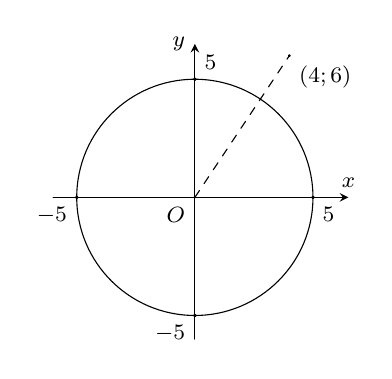
\begin{tikzpicture}[font=\footnotesize,line join=round, line cap=round, >=stealth,scale=0.3]
\draw[->] (-6,0)--(0,0)node[below left]{$O$} --(6.5,0)node[above]{$x$};
\draw[->] (0,-6) -- (0,6.5) node[left]{$y$};
\coordinate (O) at (0,0)  ;
\coordinate (A) at (4,6);
\fill (O) circle (1.5pt);
\draw[fill=black] (A) circle (1pt) node [below right] {$(4;6)$};
\draw (O) circle (5);
\draw[dashed] (O)--(A);
\draw[fill=black] (5,0) circle (1.5pt) node [below right] {$5$};
\draw[fill=black] (-5,0) circle (1.5pt) node [below left] {$-5$};
\draw[fill=black] (0,5) circle (1.5pt) node [above right] {$5$};
\draw[fill=black] (0,-5) circle (1.5pt) node [below left] {$-5$};
\end{tikzpicture}
\end{center}
\shortans[]{$2{,}21$} %Chuẩn hóa ko quá 4 ký tự
\loigiai{
\begin{center}
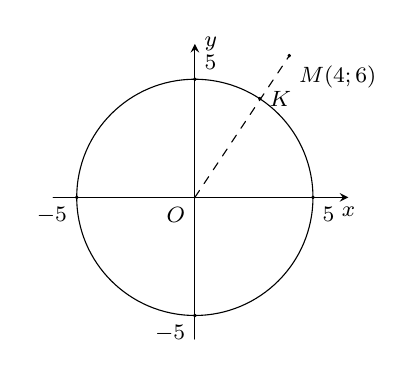
\begin{tikzpicture}[font=\footnotesize,line join=round, line cap=round, >=stealth,scale=0.3]
\draw[->] (-6,0)--(0,0)node[below left]{$O$} --(6.5,0)node[below]{$x$};
\draw[->] (0,-6) -- (0,6.5) node[right]{$y$};
\coordinate (O) at (0,0)  ;
\coordinate (A) at (4,6);
\draw[fill=black] (A) circle (1.5pt) node [below right] {$M(4;6)$};
\draw (O) circle (5);
\fill (O) circle (1.5pt);
\draw[fill=black] (5,0) circle (1.5pt) node [below right] {$5$};
\draw[fill=black] (-5,0) circle (1.5pt) node [below left] {$-5$};
\draw[fill=black] (0,5) circle (1.5pt) node [above right] {$5$};
\draw[fill=black] (0,-5) circle (1.5pt) node [below left] {$-5$};
\draw[dashed] (O)--(A);
\draw[fill=black] (2.75,4.18) circle (1.5pt) node [right] {$K$};
\end{tikzpicture}
\end{center}
Gọi $M(4;6)$, $K$ là giao điểm của $OM$ và đường tròn.\\
Khi đó khoảng cách ngắn nhất từ $M$ đến đường tròn là
\begin{align*}
MK=OM-OK=\sqrt{4^2+6^2}-5=\sqrt{52}-5\approx2{,}21.
\end{align*}
}
\end{ex}

\begin{ex}%[10-11EX-GK2 24-25]%[Lương Như Quỳnh]%[0H9H3-2]
\begin{enumerate}
\item Lập phương trình tổng quát của đường thẳng $\Delta$ biết $\Delta$ qua $M(-1;4)$ và vuông góc với đường thẳng \[d\colon\heva{&x=1+3t\\&y=5+2t}\,(t \in \mathbb{R}).\]
\item Cho tam giác $ABC$ với $A(-3;3)$, $B(1;4)$, $C(2;-5)$. Lập phương trình tổng quát đường cao $BH$ của $\triangle ABC$.
\end{enumerate}
\loigiai
{
\begin{enumerate}
\item Ta có một véc-tơ chỉ phương của đường thẳng $d$ là $\overrightarrow{u}_d=(3;2)$.\\
Vì $\Delta \perp d$ nên một véc-tơ pháp tuyến của đường thẳng $\Delta$ là $\overrightarrow{n}_\Delta=\overrightarrow{u}_d=(3;2)$.\\
Phương trình tổng quát đường thẳng $\Delta\colon 3(x+1)+2(y-4)=0 \Leftrightarrow 3x+2y-5=0$.
\item Ta có $\overrightarrow{AC}=(5;-8)$ là một véc-tơ pháp tuyến của $BH$.\\
Phương trình đường thẳng $BH$ là
$5(x-1)-8(y-4)=0\Leftrightarrow 5x-8y+27=0$.
\end{enumerate}
}
\end{ex}

\begin{ex}%[10-11-12EX-HK1-2425]%[Lê Quốc Hiệp]%[0H9H4-2]
Trong mặt phẳng $Oxy$, cho hai điểm $A(-4; -6)$ và $B(7; -1)$. Viết phương trình đường tròn $(C)$ nhận $AB$ là đường kính.
\loigiai
{
Đường tròn $(C)$ có tọa độ tâm $I$ là trung điểm của đoạn thẳng $AB$ với $I=\left(\dfrac{-4+7}{2};\dfrac{-6+(-1)}{2}\right)=\left(\dfrac{3}{2};-\dfrac{7}{2}\right)$.\\
Bán kính $R=\dfrac{AB}{2}=\dfrac{\sqrt{(7+4)^2+(-1+6)^2}}{2}=\dfrac{\sqrt{146}}{2}$.\\
Phương trình đường tròn $(C)$ có dạng
$\left(x-\dfrac{3}{2}\right)^2+\left(y+\dfrac{7}{2}\right)^2=\left(\dfrac{\sqrt{146}}{2}\right)^2\Leftrightarrow \left(x-\dfrac{3}{2}\right)^2+\left(y+\dfrac{7}{2}\right)^2=\dfrac{73}{2}.$
}
\end{ex}

\begin{ex}%[0H9V4-7]%[Dự án đề kiểm tra Toán 10 HKII NH23-24 - Dot15 - Nguyễn Ngọc Huy Trường]%[THPT Thăng Long - Tp HCM]
\immini{Hình vẽ bên mô phỏng một khu vực được bao quanh bởi một hàng rào hình tròn tại tâm $O$ có toạ độ $(0;0)$ trong mặt phẳng toạ độ (đơn vị trên hai trục là mét). Tính theo đường chim bay, xác định khoảng cách ngắn nhất để một người ở vị trí có toạ độ $(4;6)$ di chuyển được tới khu vực trong hàng rào hình tròn theo đơn vị mét (làm tròn kết quả đến hàng phần trăm). Biết rằng hàng rào hình tròn có bán kính $5$ m.
}{
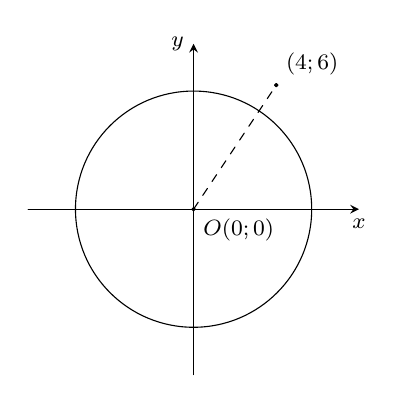
\begin{tikzpicture}[scale=0.6, font=\footnotesize,line join=round, line cap=round, >=stealth]
\def\r{2.5};
\draw[->] (-3.5,0)--(3.5,0) node[below] {$x$};
\draw[->] (0,-3.5)--(0,3.5) node[left] {$y$};
\draw[fill=black] (0,0) circle (1pt) node[below right] {$O(0;0)$};
\draw[fill=black] (1.75,2.625) circle (1pt) node[above right] {$(4;6)$};
\draw[dashed] (0,0)--(1.75,2.625);
\draw (0,0) circle (\r);
\end{tikzpicture}
}
\loigiai{
\immini{
Gọi $A(4,6)$ là điểm biểu diễn cho vị trí của người đó và gọi $(S)$ là đường tròn tâm $O$ bán kính $5m$.\\
Ta có $\vv{OA}=(4,6)$ suy ra
\[OA=\left|\vv{OA}\right|=\sqrt{4^2+6^2}=2\sqrt{13}.\]
Ta thấy $OA= 2\sqrt{13} > 5 = R$, tức $A$ nằm phía bên ngoài hàng rào hình tròn tâm $O$ bán kính $5$ m.\\
Xét $M(x,y)$ là điểm biểu diễn vị trí người đó di chuyển đến khu vực trong hàng rào, khi đó điểm $M$ sẽ nằm trong hoặc trên đường tròn tâm $O$ bán kính $5$ m, tức $OM \leq 5$.
}{\begin{tikzpicture}[scale=0.8, font=\footnotesize,line join=round, line cap=round, >=stealth]
\def\r{2.5};
\draw[->] (-3.5,0)--(3.5,0) node[below] {$x$};
\draw[->] (0,-3.5)--(0,3.5) node[left] {$y$};
\path 	(0,0) coordinate (O)
(1.75,2.625) coordinate (A)
(30:\r) coordinate (M);
\draw[name path=c1] (O) circle (\r);
\draw[dashed,name path=oa] (O)--(A);
\path[name intersections={of=c1
and oa}] (intersection-1) coordinate (M0);
\draw[fill=black] (O) circle (1pt) node[below right] {$O(0;0)$};
\draw[fill=black] (A) circle (1pt) node[above right] {$A(4;6)$};
\draw[fill=black] (M) circle (1pt) node[right] {$M(x;y)$};
\draw (O)--(M)--(A);
\draw[fill=black] (M0) circle (1pt) node[left] {$M$};
\end{tikzpicture}
}
Xét tam giác $OMA$, theo bất đẳng thức tam giác ta có $MA \leq OA - OM = 2\sqrt{13} - 5$.\\
Dấu bằng xảy ra khi và chỉ khi ba điểm $O$, $M$, $A$ thẳng hàng, tức $M$ là giao điểm của $OA$ và đường tròn $(S)$. \\
Vậy khoảng cách ngắn nhất để người đó đến khu vực trong hàng rào là $2\sqrt{13} - 5\approx 2{,}21$.
}
\end{ex}
\Closesolutionfile{ans}